
\chapter{Investigating the Separation of Salience and Valence in Implicit Cursor Control}
\chaptermark{Salience versus Valence}%
\label{chapter:salval}%


{\chaptermeta 

\textbf{Krol, L. R.\textsuperscript{1}, Pawlitzki, J.\textsuperscript{1} \& Gramann, K.\textsuperscript{1,2,3}, \& Zander, T. O.\textsuperscript{4}}

{\small
\textsuperscript{1}Biological Psychology and Neuroergonomics, Technische Universität Berlin, Berlin, Germany
\textsuperscript{2}School of Computer Science, Faculty of Engineering and Information Technology, University of Technology Sydney, Sydney, Australia
\textsuperscript{3}Center for Advanced Neurological Engineering, University of California San Diego, San Diego, CA, USA
\textsuperscript{4}Zander Laboratories B.V., Amsterdam, the Netherlands

This is a preprint version of the manuscript submitted as:

Krol, L. R., Pawlitzki, J., Gramann, K. \& Zander, T. O. (submitted). Investigating the separation of salience and valence in implicit cursor control. \textit{Proceedings of the National Academy of Sciences}.
\par}}


\abstract%
Implicit cursor control based on medial prefrontal cortex (mPFC) activity was demonstrated in 2016 \cite{zander2016nat}: neuroadaptive technology based on passive brain-computer interfacing enabled participants to essentially steer a cursor towards a highlighted target without these participants being aware of doing so. Such forms of implicit interaction can potentially enable a wide range of neuroadaptive applications, depending on which cognitive and affective processes can be reliably targeted by the classifiers that decode the corresponding brain activity. The mPFC activity in question was assumed to reflect predictive processes influenced by top-down biases informed by the participants' subjective intentions to reach the target. However, since the target was visually highlighted, it is conceivable that perceptual processes, which may be agnostic to the meaning of the visual stimuli, played a role as well. Here, we use classifier visualisation in 3D source space and an adapted experimental design to disentangle the contributions of perceptual salience- and subjective valence-related processes in implicit cursor control. We show that the two processes are both present in the data. The visualisation method allows them to be separated and localised in different cortical areas, with visual processing primarily situated in parietal areas and valence-related processing predominantly in the mPFC. This also demonstrates that neuroadaptive technology can indeed access subjective valence-related processes for implicit control.


\clearpage


\fancypagestyle{salval}{%
    \fancyhf{}
    \fancyhead[EC]{\textit{\leftmark}}
    \fancyhead[OC]{\textit{\rightmark}}
    \fancyfoot[C]{\thepage \\ \vspace{9.9mm} \colorbox{footerbg}{\parbox{\paperwidth-2\fboxsep}{\centering\parbox{0.75\paperwidth}{\centering\fontsize{9pt}{9pt}\selectfont\textcolor{footerfg}{This is a preprint version of submitted manuscript: Krol, L. R., Pawlitzki, J., Gramann, K. \& Zander, T. O. (submitted). Investigating the separation of salience and valence in implicit cursor control. \textit{Proceedings of the National Academy of Sciences}.}}}}}
    \fancyfootoffset[]{1.25in}
}
\pagestyle{salval}


\section{Introduction}

A brain-computer interface (BCI) allows a measurement of a person's brain activity to be interpreted in real time and used as input to a computer, essentially providing a new communication channel that does not depend in any way on muscular activity \cite{wolpaw2012newsun}. While the focus of BCI research has long been on medical applications, for example offering paralysed patients the ability to communicate with the outside world or control parts of their environment \cite{birbaumer2006commcontrol,vansteensel2016alsimplant},
the scope of BCI technology has significantly widened in roughly the past decade with hard- and software solutions now being offered even to the general public \cite{ienca2018brainleaks}. Of particular note is the category of so-called \emph{passive} BCI systems (pBCI; \citeNP{zander2011,krol2018interactivity}), which are different from other categories of BCI in that they derive output from brain activity that was not specifically modulated for communication or control. Instead, pBCI decodes a person's naturally occurring brain activity, thus revealing aspects of their naturally occurring mental states. This decoded \emph{implicit input} can potentially be obtained without the user's explicit voluntary cooperation \cite{schmidt2000,rotting2009implicit,zander2014implicit}. As such, a pBCI could for example allow a smart car to detect its driver's state of drowsiness and automatically pull over without requiring the drowsy driver to make any explicit decisions \cite{zander2017dry}, or allow adaptive systems to respond to different levels of their users' mental load without adding any additional load to it \cite{yuksel2016bach,ewing2016tetris,zander2017surgery}. Such systems using implicit input in order to adapt themselves, e.g. for control or interaction, are referred to as neuroadaptive technology \cite{zander2016nat}.

In the context of human-computer interaction, the operator's naturally occurring brain activity is largely dependent on current task parameters. Neuroadaptive technology can automatically adapt these parameters in order to support the human operator, but conversely, it can also pro-actively change these parameters in order to induce specific mental states, or to learn from the brain activity resulting from specific changes. For example, rather than increasing or decreasing automation levels in response to rising or lowering levels of workload \cite<e.g.,>{byrne1996adaptiveauto}, a system could actively cycle through a set of possible task configurations in order to evaluate which produces the optimal level of load. This method is called cognitive probing \cite{krol2020cognitiveprobing}.

In an earlier work, we demonstrated how cognitive probing can be used to enable implicit cursor control \cite{zander2014implicit,zander2016nat}. Where traditional forms of BCI can enable users to steer a cursor by actively producing different mental states (most commonly, this is motor imagery; \citeNP{pfurtscheller2001motorimagery}), the implicit cursor control paradigm started with a cursor that was moving autonomously, but randomly, across the nodes of a grid. One of the corners of this grid was visually highlighted to represent the target, i.e., the supposed goal of the cursor's movements. Participants were instructed to judge each individual cursor movement as being either `appropriate' or not with respect to reaching the indicated target. The results showed significant differences between (appropriate) cursor movements going towards the target, and (inappropriate) movements leading the cursor away from the target. Furthermore, this difference was classifiable with an estimated single-trial accuracy of 72\%. We could thus use this classifier output in real time as implicit input, in order to reinforce the initially random cursor movements to gradually guide the cursor towards the target. When brain activity indicated that a movement was appropriate, the probability of moving again in that same direction was increased, and conversely, the corresponding probability was decreased after each movement that was classified as inappropriate. This produced significantly goal-directed behaviour of the cursor, purely on the basis of brain activity elicited by each and every movement. A similar concept was demonstrated by \citeA{iturrate2015teaching}. We emphasise, however, that in \citeA{zander2016nat}, the participants were unaware of having any influence on the cursor's movements, hence this being an example of implicit control.

An analysis of the signal underlying classification in this implicit cursor control experiment revealed the relevant cognitive processes to stem predominantly from the medial prefrontal cortex (mPFC). In particular, inappropriate movements elicited a strong negativity visible at channel Fz around 180~ms. This and various additional findings led to these results being interpreted within the framework of predictive coding: the brain's automatic, constant prediction of future sensory input in order to optimise behaviour by minimising prediction errors \cite{friston2010free,clark2013predictive}. Processes with a similar time course, spatial distribution, and cortical origin have been identified to be involved in the realisation of having committed an error \cite{falkenstein1990,falkenstein2000}, receiving feedback concerning previous errors \cite{miltner1997,holroyd2003frn}, receiving feedback concerning erroneously executed commands \cite{ferrez2008simulated,mousavi2017mi}, and observing others commit errors \cite{miltner2004,schie2004}. Their many similarities have resulted in the assumption that these negativities are generated by the same system, but under different circumstances; in particular, the \emph{error-related negativity} is said to follow actively committed errors, while the \emph{feedback-related negativity} follows the display of performance-related feedback \cite{walsh2012frnreview}. An account based on reinforcement learning has therefore been postulated which holds that a generic error-processing mechanism exists, in which changes in the dopaminergic input to the anterior cingulate cortex (ACC) indicate whether or not predictions have been met \cite{holroyd2002,nieuwenhuis2004rlern}. At the scalp, this activity is then reflected as a negativity in case of events being worse than predicted, and/or a positivity when events are better than predicted \cite{holroyd2008rewardpositivity}. 

Therefore, we hypothesised that participants in the implicit cursor control paradigm predicted that the cursor would move towards the target, with correct movements towards the target (i.e., positive feedback) yielding the known positivity and incorrect movements the corresponding negativity. In the absence of any informative cues with respect to upcoming cursor movements, the participants' intentions or preferences pertaining to the cursor movements thus determined how each movement was predicted and interpreted. As such, higher-order cognitive functions (here: intentions or preferences) could be inferred from lower-level processes (predictive error signals). Such lower-level processes may be difficult to consciously control, with potentially far-reaching implications for the privacy of thought \cite{mecacci2019criteria}.

The feedback-related negativity is generally considered to be a binary signal reflecting the processing of positive or negative outcomes, influenced by motivational involvement but not by reward or error magnitude \cite{yeung2004passiveactivefrn,hajcak2006binaryfrn}. Interestingly, the negativity observed in the implicit cursor control paradigm showed a linear dependency on the `appropriateness' of the cursor movements, as measured by their angular deviance from a straight line towards the target. This hinted at the involvement of a cortical process that not only signals deviations from predicted events in order to improve future behaviour, but in fact confirms or rejects predictions in a graded way in order to e.g. reinforce adequate behaviour or sharpen perceptive hypotheses. Combined with the above-mentioned assumption that these predictions are informed by higher-level cognition, this process would then essentially reflect a subjective degree of goal attainment.

However, this interpretation assumes that there indeed was no other information available---even false information---to base a prediction on. As mentioned, in the implicit cursor control experiment the desired target was visually highlighted, thus potentially making this a form of information: it is visually more salient than other nodes in the grid, and thus, it is conceivable that perceptive processes would interpret this as a reference point regardless of its valence. It is conceivable that a `default' prediction is for one salient object (the cursor) to move towards another salient object (the target).

In light of this, a more nuanced perspective has been suggested to interpret the detected event-related potentials (ERPs) \cite{cockburn2018rewardpositivity}. Holroyd and colleagues make a distinction between surprise- or salience-related signals on the one hand, the response of which is modulated by the expectancy of events \cite{holroyd2002}, and the \emph{reward prediction error} signal on the other hand, which responds most strongly to unexpected (i.e. surprising, salient) events but whose sign is inverted for positive versus negative events \cite{sambrook2015rewardprediction}. This has primarily been investigated in the context of tasks where a positive event would for example indicate correct performance or monetary reward on a timing or gambling task, but may also apply to implicit cursor control. In short, while the different valence of movements towards and away from the target should result in a classifiable signal, the visual salience of these same movements towards or away from the highlighted node may confound these results. It thus remains an important unanswered question to what extent the signal that allowed classification may also have ``[manifested] as a specific interaction between outcome valence and outcome probability'' \cite{heydari2016rewardorsalience}, or indeed, may be explained exclusively by one or the other.

To be specific, we understand `salience' in the context of implicit cursor control to represent the perceptual (here: visual) properties of the cursor movements relative to the visually salient point of the grid. `Valence' on the other hand is the meaning imparted upon these movements by the participants as informed by the instructions, leading participants to see some movements as `appropriate' (positive valence) and others as `inappropriate' (negative valence). Because salience and valence of the cursor's movements were coupled in the original implicit cursor control experiment, it was not possible for these two factors to be differentiated. We therefore conducted a similar but adapted experiment where the visual stimuli and the participants' task were designed to allow such a differentiation to be made. In the updated design, visual stimuli were left constant between two conditions that differed only with respect to the given instructions. These instructions manipulated the valence of the visually identical stimuli. 

If processes related to visual salience were the sole or primary cause of the effects seen in the original paradigm, we should see the same effects in this experiment in both conditions. Conversely, if valence-related processes were primarily driving the results, we would expect to see an inverse pattern between the two conditions. In case both of these dimensions play a role, as is most probable, the updated experimental design allows us to compare valence parameters while isolating or controlling for visual parameters, and vice versa. This would allow us to identify which cortical areas primarily contribute to these two aspects. Here, we would expect salience to be localised primarily in occipital/parietal regions, and valence in the mPFC as per the original results.

Aside from further elucidating the neurophysiology of error- and feedback-related processing, it is important to investigate salience- and valence-related processes in the context of neuroadaptive technology. A classifier that responds only to physical (e.g. visual, salience) parameters while being agnostic to more subjective cognitive processes may have a limited number of applications in the real world. On the other hand, when a system does have access to its user's subjective (valence-related) processing, care must be taken that both this access and the gathered information is handled with due care---among other things, keeping in mind the necessity for informed consent and the value of privacy. See \citeA{krol2020cognitiveprobing} for a discussion on the ethical implications of some forms of neuroadaptive technology, which are all the more pertinent when subjective interpretations can inform the adaptations, as opposed to more `neutral' cognitive processes such as perception.


\section{Methods}

\subsection{Participants and Set-Up}

A total of 24 participants participated in the study (10 male; 22 right-handed; mean age $26.6\pm3.9$). All signed a written informed consent form. 64-channel EEG was recorded at 5000~Hz using BrainAmp DC amplifiers (Brain Products GmbH, Gilching, Germany), with active electrodes arranged on actiCAP electrode caps according to the extended international 10-20 system, referenced to FCz. Participants were seated in front of a 27'' computer display placed approximately 1~m away from them. Five participants were later excluded from the analysis due to data quality or recording issues, leaving 19 datasets (9 male; 17 right-handed; mean age $26.6\pm4.3$).


\subsection{Experimental Paradigm}

The experimental paradigm largely followed the original implicit cursor control experiment \cite{zander2014implicit,zander2016nat}, but with adaptations to allow salience and valence to be manipulated as independent variables. This required a different grid layout, shown in figure~\ref{salval:fig:grid}.

\begin{figure}[t]
    \centering
    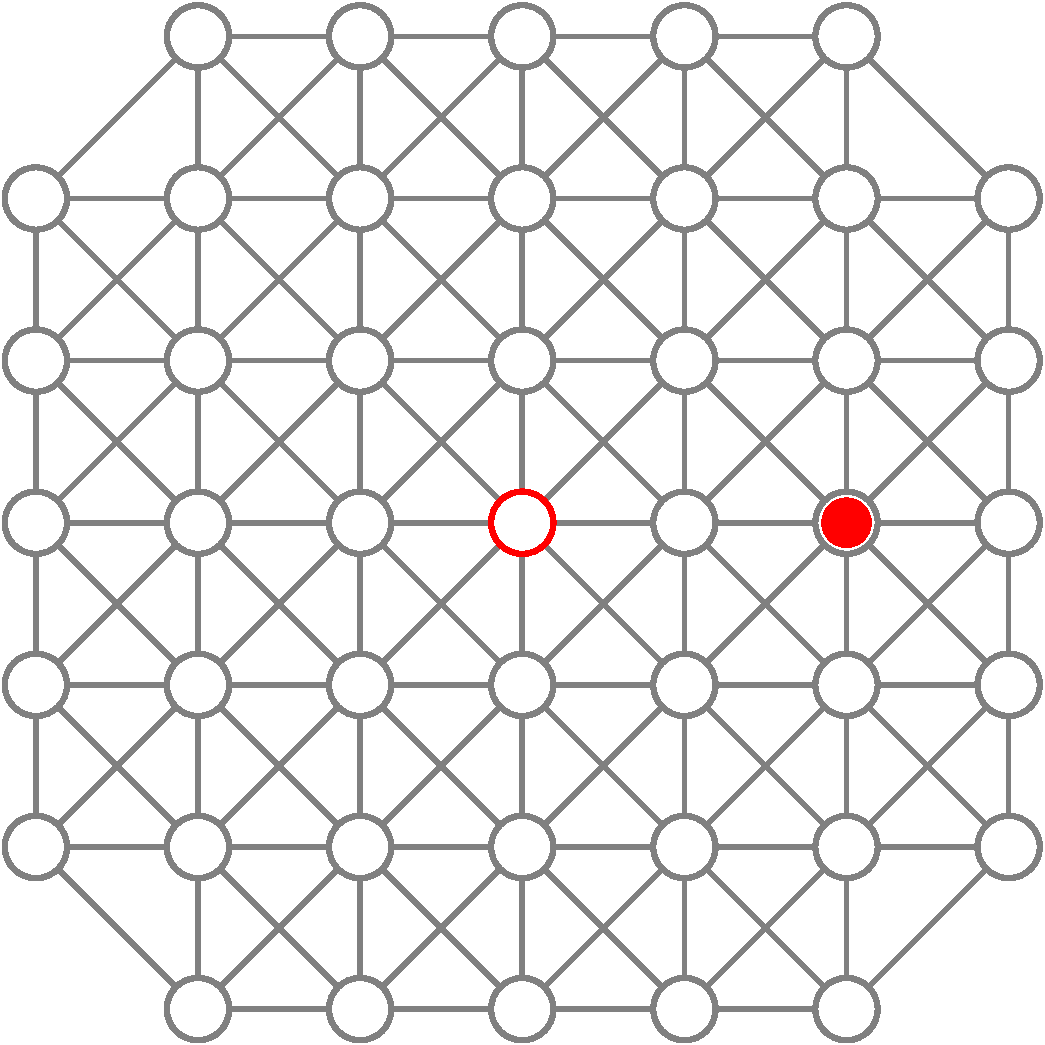
\includegraphics[width=0.5\textwidth]{figures/salval-grid.pdf}
    \caption{The grid layout as seen by the participants, with the cursor at one of four possible starting positions. The centre node was always visually highlighted.}
    \label{salval:fig:grid}
\end{figure}

The original experiment used a square grid with one of the corners bearing particular relevance (e.g., the target). On such a grid there is always an opposite corner that may, inversely, be interpreted as having particular relevance as well, being the furthest away from said target. In other words, instructions that assign positive or negative valence to one corner, may be mentally translated as assigning inverted valence to the opposite corner instead. Because of this, we instead used a larger $7\times7$ grid allowing us to place the reference node at the centre, and removed the corner nodes to eliminate any `opposite' candidates. All grid nodes were grey, open circles connected by grey lines. The reference node was a red, open circle. The cursor was a red, filled circle, somewhat smaller than the nodes. The background was black.

Starting two nodes away from the centre in a horizontal or vertical line, the cursor would move randomly to any of the up to eight adjacent nodes at a rate of one movement every three seconds. Each movement first consisted of a 1-second animation of a growing white `ghost' circle inside the cursor's red circle. This allowed the participants to predict the timing of the upcoming move. Upon reaching the same size as the cursor's red circle, the ghost cursor instantaneously moved to the next node while the red cursor remained. The grid line between these two points was highlighted in white, clearly indicating the movement between the previous and new cursor positions. This remained visible for 1 second. Following this, the red cursor instantaneously moved to the new position while the white elements disappeared. The red cursor remained at this position for 1 second before the next anticipatory animation started. (A video of this animation is available in \citeNP{zander2016nat}.)

In order to manipulate valence, there were two conditions: an `attraction' and a `repulsion' condition, defined relative to the reference node in the centre. In the attraction condition, participants were instructed that the cursor \emph{should} reach the centre node, and that reaching it should be seen as a success. If the cursor had not reached the centre after 50 movements, this was to be seen as a failure. These instructions reflected those of the original experiment. In the negative condition, the instructions were reversed: the cursor should \emph{not} reach the target, and was given 25 movements to either fail or succeed. The difference in the maximum number of movements was to even out the number of successes and failures per condition. After success or failure in either case, the grid was restarted with a different cursor starting position. The order of the two conditions was counter-balanced across participants. 

The two conditions inverted the valence of the otherwise visually identical stimuli: what was `appropriate' in one condition was `inappropriate' in the other. Participants were instructed to observe each cursor movement and label it as either `appropriate' or `inappropriate' given the current condition through a button press before the next movement occurred, i.e. within three seconds. Speed was not emphasised. Participants were given no explicit instructions as to what exact criteria to use for each judgement, but they were told that each judgement was to be made for the individual cursor movement, independent of the larger history of cursor movements. These individual cursor movements were the unit of analysis in this experiment.

Participants observed and evaluated a total of 800 cursor movements per condition for 1600 movements in total. Self-paced breaks were given between grids.

The cursor moved randomly throughout the experiment. There was no condition using online implicit cursor control.


\subsection{Independent Component Analysis}

Using EEGLAB 14.1.2b \cite{delorme2004eeglab}, the raw EEG data was subsampled to 250~Hz and band-pass filtered between 1 and 100~Hz. Channels were rejected using \texttt{clean\_rawdata}. Removed channels were spherically interpolated, and the data was re-referenced to the common average while maintaining full rank by first re-inserting the all-zero reference channel \cite{miyakoshi2017fullrankaveref}. After manually removing sections of the data highly contaminated by artefacts, two passes of independent component analysis (ICA; \citeNP{makeig1996}) were performed. A first pass yielded reliable identification of eye-related independent components (ICs), which were then removed to allow automated cleaning of the data without this algorithm erroneously identifying eye-related activity as noise. With noise sections identified, these were removed from the earlier dataset still containing eye activity, and a second pass of ICA yielded the decomposition used for further analysis.

The ICA algorithm used was AMICA \cite{palmer2012amica}, stopping either when convergence was reached or after 2000 iterations. The automated cleaning algorithm, described in more detail by \citeA{gramann2018heading}, first filtered the data between 1 and 40~Hz, and took the absolute value of the Hilbert transform of each channel. It then looked at 1-second non-overlapping time segments, and first removed any segment where a flat line occurred for more than 100~ms. Following this, all segments were ranked by their mean absolute amplitude across channels, their standard deviation across channel means, and their Mahalanobis distance from a distribution spanning all segments using the channel means as coordinates. The top 10\% of segments sorted by their mean rank, plus a 500-ms margin on either side, were then removed from the data.

The resulting ICs were dipole-fitted using DIPFIT 2.x \cite{oostenveld2003dipfit} matched to an MNI average head model. The EEGLAB plug-in ICLabel \cite{piontonachini2019iclabel} was used to identify components. Only `brain' components were kept, defined as having a residual variance of less than 15\% and a `brain' probability of at least 67\%. Non-brain components were removed. For a cluster inspection, the remaining brain ICs were clustered based on their dipole positions (relative weight in the preclustering array: 10), ERP activities (weight 1), and scalp maps (weight 1). Clustering was done using k-means producing 15 clusters, with an outlier threshold at 3 standard deviations.


\subsection{Classification}
\label{salval:sec:methods:classification}

The experiment essentially resulted in $2\times2$ classes: each movement could be categorised by visual salience as either going `towards' or `away' from the centre, or by valence as either being `good' or `bad' in the given condition. `Towards' and `away' were defined using the movements' angular deviance from a straight line towards the centre. For example, a movement with an angular deviance of $0^{\circ}$ goes directly towards the centre; a movement with an angular deviance of $180^{\circ}$ moves in a straight line away from the centre. Following calculations regarding class separability depending on different definitions of `towards' and `away', done on the first eight participants \cite{krol2019saliencevalence}, movements having an angular deviance of $\leq27^{\circ}$ were labelled as going `towards' the target, while $>117^{\circ}$ were `away'. The attraction condition thus contains \emph{good-towards} and \emph{bad-away} movements, whereas the repulsion condition contains \emph{good-away} and \emph{bad-towards} movements.

Classification was implemented using BCILAB \cite{kothe2013bcilab}. After downsampling the data to 100~Hz and band-pass filtering it between 1 and 15~Hz, we used a windowed-means approach \cite{blankertz2011} taking the mean amplitude on all channels in twelve non-overlapping 50-ms time windows ranging from 0 to 600~ms as features. This large range was chosen to include both early perceptual and later semantic processing. Linear discriminant analysis (LDA; \citeNP{bishop2006}) was used to calibrate the classifier. Five-fold random cross-validation was used to estimate classifier accuracy. Since all four classes were equalised by randomly eliminating trials from larger classes, this whole procedure was repeated five times and the reported values represent the mean across iterations.

We always classified one class of movements against one other. Within conditions, this would thus be good-towards versus bad-away for the attraction condition (Att.), and bad-towards versus good-away for the repulsion condition (Rep.). These classifications combine both valence and salience factors. To separate them, four additional classifications were performed: good-towards versus bad-towards (TvT) and good-away versus bad-away (AvA) to focus on valence differences between visually identical movements, and good-towards versus good-away (TvA+) and bad-towards versus bad-away (TvA--) to focus on the visual differences while controlling for valence.


\subsection{IC Relevance Weighting and Classifier Visualisation}

The method described in detail by \citeA{krol2018classvis} was used to obtain so-called relevance weights for each IC. In short, the channel-level spatial filter weights produced by each classifier, representing the classifier's backward model, were first transformed into forward-model patterns \cite{haufe2014}. These patterns represent the projected activity of the signals isolated by the classifier. Using the unmixing matrix obtained from the ICA, these patterns were translated into source-level weights, indicating, for each IC in each of the classifier's time windows, to what extent it contributed to classification. These so-called relevance weights were normalised across time windows within participants.

Given the dipole model fitted to each IC, the IC relevance weights can be visualised in 3D source space. Using the dipoleDensity EEGLAB plug-in \cite{miyakoshi2013dipdens}, each IC's position in the average brain volume was weighted according to its relevance to classification. We then generated a weighted 3D kernel density plot containing these weights for all participants in one figure, using a smoothing kernel of 10~mm. The scales in these images are relative, as they intend to bring physiological rather than quantitative differences into focus.

% The relevance weights can also be used to generate a weighted source-level ERP reflecting the time series of the activity isolated by the classifier. To generate these, each IC time series was weighted by the IC's relevance weight, and the weighted IC activations were summed together within subjects.


\section{Results}

\subsection{Behavioural Data}

In the attraction condition, the cursor made an average of $28.4\pm3.9$ movements per grid; in the repulsion condition, this was $19.0\pm5.1$ movements per grid. The definitions used to define the `towards' and `away' classes (i.e. `appropriate' and `inappropriate' movements) resulted in a roughly similar total of 388 movements towards, and 343 away across conditions. Grand average reaction times for the button presses were $690\pm153$~ms and $731\pm175$~ms in the attraction and repulsion condition, respectively. A within-participants permutation test with 10000 permutations found that 13 participants showed significant differences ($\alpha=0.05$, Bonferroni-corrected) in their reaction times between conditions; in all these cases, the repulsion condition had longer reaction times. For the other six, no significant differences were found. We furthermore investigated reaction time differences between two groups of participants, separated by which condition was presented first. The attraction-first group was shown the attraction condition first, and the repulsion condition second; the repulsion-first group was shown the repulsion condition first, and the attraction condition second. We performed this analysis in order to detect or rule out any order effect. Permutation tests with 10000 permutations revealed no significant differences between groups for each of the condition (all $p>0.64$).


\subsection{Independent Component Analysis}

Keeping only cortical components left on average $14.2\pm4.3$ ICs per participant. For an impression of the distribution of these ICs and as a reference for the later classifier visualisation, these ICs were clustered using k-means clustering in EEGLAB 14.1.2b \cite{delorme2004eeglab} using the same information available to the classifier---the ERPs and scalp maps, each with weight 1---and the dipole locations, with weight 10, with the threshold for outliers set at 3 standard deviations. Figure~\ref{salval:fig:clusters} shows both the dipole distribution and the scalp maps of the clusters.

\begin{figure}[htb]
    \centering
    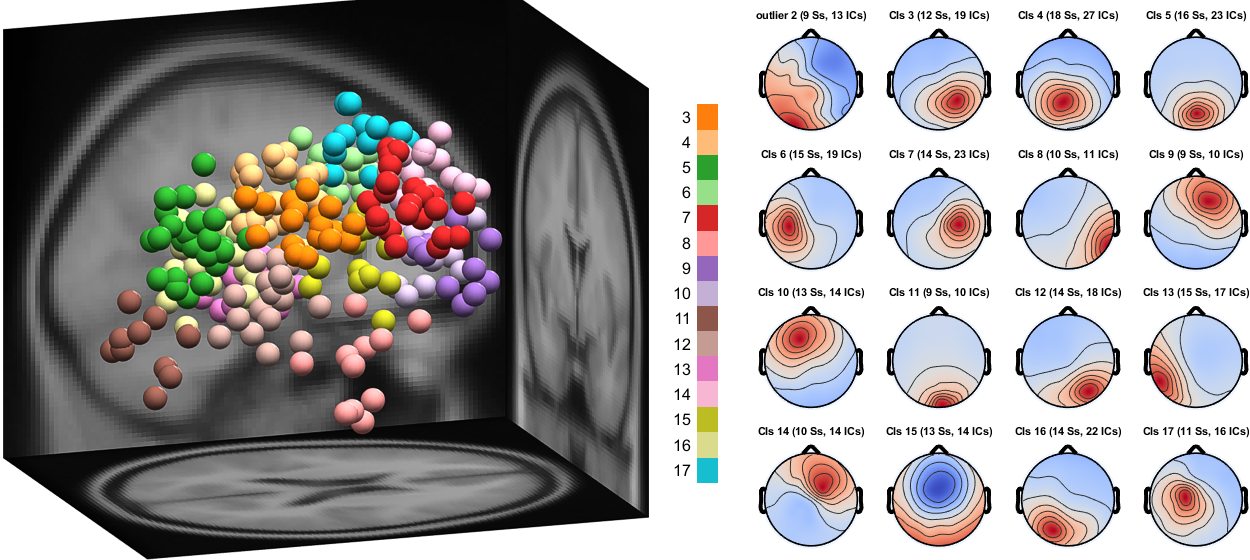
\includegraphics[width=\textwidth]{figures/salval-clusters.png}
    \caption[Independent component dipoles and cluster scalp maps.]{\emph{Left:} All 257 cortical ICs, colour-coded for each cluster, excluding 13 outlier ICs. \emph{Right:} The mean scalp maps of all 15 clusters, plus the outlier cluster.}
    \label{salval:fig:clusters}
\end{figure}


\subsection{Classification}

Table~\ref{salval:tab:bci} contains the cross-validated accuracy estimations for the six different classification schemes, using only cortical ICs. Removing non-brain ICs reduced the classification accuracy by a moderate 2.24 percentage points on average, a reduction which was nonetheless significant in most cases following paired-sample t-tests (Att $p=0.300$, Rep $p=0.011$, TvT $p=0.002$, AvA $p=0.001$, TvA+ $p=0.001$, TvA-- $p=0.003$). Still, classification accuracies for the vast majority of participants remained significantly above chance. Since the number of trials for each class was equalised, chance level is at 50\%. Classification rates that are significantly better than chance, adjusted for the number of trials \cite{mullerputz2008random}, are indicated in the table.


\begin{table}[p]
    \renewcommand{\arraystretch}{0.85}
    \centering
    \begin{tabular}{rllllll}
        \textbf{Participant}& \textbf{Att}       & \textbf{Rep}       & \textbf{TvT}      & \textbf{AvA}      & \textbf{TvA+}     & \textbf{TvA--}    \\
        1$^r$               & 85{\tiny$^{***}$}  & 68{\tiny$^{***}$}  & 63{\tiny$^{***}$} & 67{\tiny$^{***}$} & 80{\tiny$^{***}$} & 80{\tiny$^{***}$} \\
        2$^a$               & 66{\tiny$^{***}$}  & 61{\tiny$^{***}$}  & 57{\tiny$^{*}$}   & 59                & 69{\tiny$^{***}$} & 69{\tiny$^{***}$} \\
        3$^r$               & 77{\tiny$^{***}$}  & 64{\tiny$^{***}$}  & 62{\tiny$^{***}$} & 55{\tiny$^{***}$} & 74{\tiny$^{***}$} & 74{\tiny$^{***}$} \\
        4$^a$               & 80{\tiny$^{***}$}  & 75{\tiny$^{***}$}  & 67{\tiny$^{*}$}   & 67{\tiny$^{***}$} & 81{\tiny$^{***}$} & 81{\tiny$^{***}$} \\
        5$^r$               & 76{\tiny$^{***}$}  & 68{\tiny$^{***}$}  & 57{\tiny$^{***}$} & 59{\tiny$^{**}$}  & 70{\tiny$^{***}$} & 70{\tiny$^{***}$} \\
        6$^a$               & 88{\tiny$^{***}$}  & 74{\tiny$^{***}$}  & 70{\tiny$^{***}$} & 77{\tiny$^{***}$} & 78{\tiny$^{***}$} & 78{\tiny$^{***}$} \\
        7$^r$               & 82{\tiny$^{***}$}  & 66{\tiny$^{***}$}  & 60{\tiny$^{***}$} & 62{\tiny$^{***}$} & 71{\tiny$^{***}$} & 71{\tiny$^{***}$} \\
        8$^a$               & 78{\tiny$^{***}$}  & 60{\tiny$^{***}$}  & 65{\tiny$^{***}$} & 61{\tiny$^{***}$} & 72{\tiny$^{***}$} & 72{\tiny$^{***}$} \\
        10$^r$              & 72{\tiny$^{***}$}  & 61{\tiny$^{***}$}  & 65{\tiny$^{***}$} & 70{\tiny$^{***}$} & 55{\tiny$^{*}$}   & 55{\tiny$^{***}$} \\
        11$^a$              & 76{\tiny$^{***}$}  & 66{\tiny$^{***}$}  & 58{\tiny$^{**}$}  & 57{\tiny$^{**}$}  & 76{\tiny$^{***}$} & 76{\tiny$^{***}$} \\
        13$^r$              & 84{\tiny$^{***}$}  & 65{\tiny$^{***}$}  & 62{\tiny$^{***}$} & 61{\tiny$^{***}$} & 77{\tiny$^{***}$} & 77{\tiny$^{***}$} \\
        14$^a$              & 71{\tiny$^{***}$}  & 56                 & 66{\tiny$^{***}$} & 63{\tiny$^{***}$} & 68{\tiny$^{***}$} & 68{\tiny$^{**}$}  \\
        15$^a$              & 86{\tiny$^{***}$}  & 68{\tiny$^{***}$}  & 67{\tiny$^{***}$} & 64{\tiny$^{***}$} & 79{\tiny$^{***}$} & 79{\tiny$^{***}$} \\
        16$^r$              & 69{\tiny$^{***}$}  & 60{\tiny$^{***}$}  & 59{\tiny$^{***}$} & 58{\tiny$^{**}$}  & 73{\tiny$^{***}$} & 73{\tiny$^{***}$} \\
        17$^a$              & 78{\tiny$^{***}$}  & 69{\tiny$^{***}$}  & 65{\tiny$^{***}$} & 71{\tiny$^{***}$} & 68{\tiny$^{***}$} & 68{\tiny$^{***}$} \\
        20$^r$              & 85{\tiny$^{***}$}  & 59{\tiny$^{***}$}  & 66{\tiny$^{***}$} & 66{\tiny$^{***}$} & 73{\tiny$^{***}$} & 73{\tiny$^{***}$} \\
        21$^a$              & 69{\tiny$^{***}$}  & 58{\tiny$^{**}$}   & 56{\tiny$^{*}$}   & 56{\tiny$^{*}$}   & 69{\tiny$^{***}$} & 69{\tiny$^{***}$} \\
        22$^r$              & 82{\tiny$^{***}$}  & 70{\tiny$^{***}$}  & 61{\tiny$^{***}$} & 68{\tiny$^{***}$} & 76{\tiny$^{***}$} & 76{\tiny$^{***}$} \\
        24$^r$              & 59{\tiny$^{***}$}  & 61{\tiny$^{***}$}  & 63{\tiny$^{***}$} & 61{\tiny$^{***}$} & 71{\tiny$^{***}$} & 71{\tiny$^{***}$} \\
        \textbf{Mean}       & \textbf{77}        & \textbf{65}        & \textbf{63}       & \textbf{63}       & \textbf{73}       & \textbf{71}       \\
        \textbf{Mean sig.}  & \textbf{77}        & \textbf{66}        & \textbf{64}       & \textbf{66}       & \textbf{74}       & \textbf{71}       \\
    \end{tabular}
    \caption[Classification accuracies.]{Classification accuracies (\%) for the separability of the following classes. Att: towards v away in the attraction condition, i.e. good-towards v bad-away; Rep: towards v away in the repulsion condition, i.e. bad-towards v good-away; TvT: towards v towards across conditions, i.e. good-towards v bad-towards; AvA: away v away across conditions, i.e. good-away v bad-away; TvA+: towards v away with positive valence across conditions, i.e. good-towards v good-away; TvA--: towards v away with negative valence across conditions, i.e. bad-towards v bad-away. For the participants, \emph{a} or \emph{r} indicate that the attraction or repulsion condition was presented first, respectively. Significance is indicated as *~$\scriptstyle{p<0.05}$, **~$\scriptstyle{p<0.01}$, ***~$\scriptstyle{p<0.001}$. Mean sig. indicates the mean accuracy taking only those participants with $\scriptstyle{p<0.001}$.}
    \label{salval:tab:bci}
\end{table}

Separation between the classes is significantly better for Att than for Rep ($p<0.001$ using paired-sample t-tests). TvT does not significantly differ from AvA ($p=0.275$), nor does TvA+ from TvA-- ($p=0.047$). Att is significantly better than the four mixed-condition classification schemes (TvT $p<0.001$, AvA $p<0.001$, TvA+ $p<0.001$, TvA-- $p<0.001$); Rep is significantly worse than TA+ ($p=0.001$) and TA-- ($p<0.001$) but does not differ significantly from TvT ($p=0.758$) or AvA ($p=0.956$). 

Also here, we investigated differences between the attraction-first and repulsion-first groups in order to detect or rule out any order effect. Permutation tests with 10000 permutations comparing the accuracies of six classification schemes across groups revealed no significant differences (all $p>0.26$).

\begin{figure}[p]
    \centering
    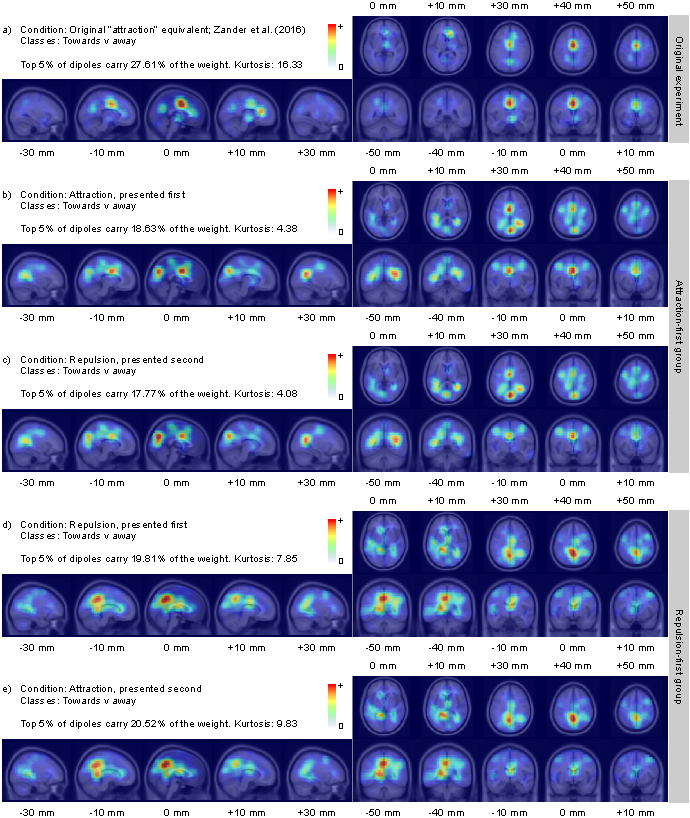
\includegraphics[width=\textwidth]{figures/salval-wdd-within.pdf}
    \caption[Weighted dipole density plots for the within-condition classifiers.]{Weighted dipole density plots showing the relevance of cortical areas to \emph{a} the original implicit cursor control experiment's classifier, \emph{b} the Att classifier for participants who saw the attraction condition first, \emph{c} the Rep classifier for the same group, \emph{d} the Rep classifier for participants who saw the repulsion condition first, and \emph{e} the Att classifier for the same group.}
    \label{salval:fig:wdd-within}
\end{figure}


\subsection{Single-Condition Classifier Visualisation}

Figure~\ref{salval:fig:wdd-within} illustrates the source-localised relevance weights for the Att and Rep classifiers, as well as for the classifier from the original implicit cursor control experiment for comparison. These figures thus show which cortical sources contributed to the separability of the classes within conditions. For increased sensitivity, each plot only includes participants for whom the respective classifier was significantly above chance at $\alpha=0.001$. Since an effect is visible here depending on which condition was presented first, the attraction-first and repulsion-first groups are separated accordingly.

Panel \emph{a} shows the relevant areas for the original experiment's classifier, equivalent to the attraction condition in this study. Panel \emph{b} and \emph{c} show the relevant areas for the current experiment's attraction and repulsion condition, respectively, but only for those participants who saw the attraction condition first. Panels \emph{d} and \emph{e} show the repulsion and attraction condition, respectively, for the remaining participants who saw the repulsion condition first. Note that all five of these classifiers combine both salience and valence dimensions. 

For the attraction-first group, the relevant cortical areas for the Att classifier largely overlap with the Att-equivalent classifier of the original experiment. There is a clear focus on the mPFC, a second focus on the centro-parietal region, albeit larger than in the original experiment, plus an additional weaker focus localised in the right-lateral parietal cortex. For the Rep classifier of the first group, these same three areas remain active, now with a stronger parietal focus than for the Att classifier.

For the repulsion-first group, for both Att and Rep classifiers, the same general centro-parietal area carries most weight with virtually no difference between the two conditions.

Interestingly, while participants within each of the two groups consistently showed relevant activations in the same areas for both conditions, the area that almost exclusively contributed to classification in the repulsion-first group, is virtually absent in any classifier of the attraction-first group, and vice versa. Given this stark difference between the two groups depending on the order of presentation, we separate the further analysis between the two groups. We will focus on the attraction-first group, as this group more closely resembles the reference data with which we wish to compare the current results. The same analysis for the repulsion-first group is provided in Section~\ref{salval:sec:results:repulsionfirst}.


\subsection{Event-Related Potential at Fz}

Figure~\ref{salval:fig:posfirst-erp-channel} shows the scalp ERP at channel Fz for the processed data, i.e., referenced to the common average, with non-cortical contributions removed, and filtered between 1 and 15~Hz. The attraction condition (when presented first), on the left panel, reproduces the result from the original experiment with a peak negativity following (negative-valence) movements away from the centre node at around 180~ms, versus a peak positivity at that same time for (positive-valence) movements towards the centre. 

\begin{figure}[htb]
    \centering
    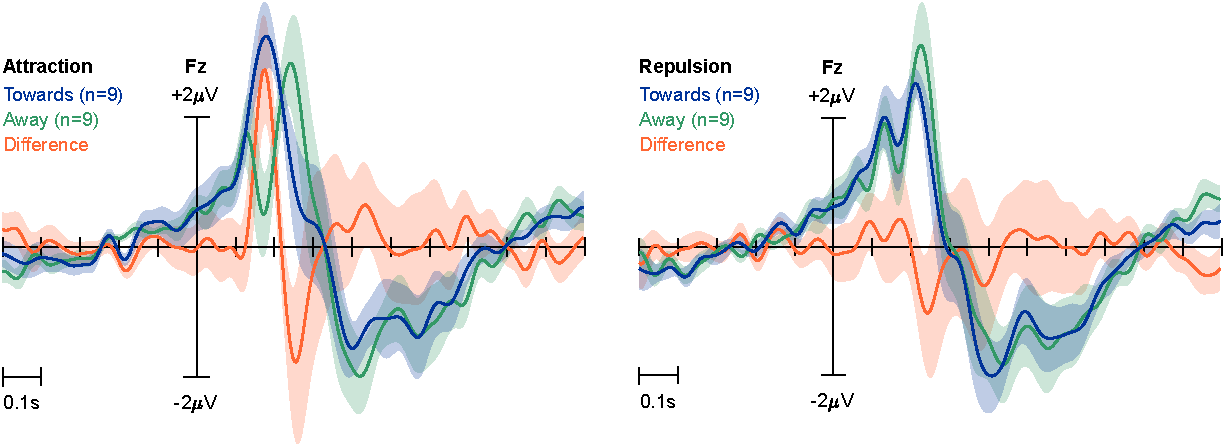
\includegraphics[width=\textwidth]{figures/salval-posfirst-erp-channel.pdf}
    \caption[The grand average ERPs at Fz for the two conditions in the attraction-first group.]{The grand average ERPs at Fz for the two conditions in the attraction-first group.}
    \label{salval:fig:posfirst-erp-channel}
\end{figure}

The repulsion condition (when presented second), however, shows neither the same nor the inverted pattern that would be indicative of salience-only or valence-only processes, respectively, being involved in its production. Rather, at around 180~ms a negative deflection can be seen in both classes. This negativity is smaller than the negativity seen in the attraction condition, with its mean amplitude holding the middle between the attraction condition's negativity and positivity.

Using permutation tests with 10000 permutations, significant differences ($p<0.05$) between the curves are found consistently between 160 and 200~ms in the attraction condition. The repulsion condition shows no significant differences between the two classes, towards and away.

\subsection{Valence- and Salience-Focused Classifier Visualisation}
\label{salval:sec:results:classvis}

Figure~\ref{salval:fig:wdd-within}, discussed above, shows the cortical areas contributing to the first two classifiers from Table~\ref{salval:tab:bci}, which include both salience and valence dimensions. The current study was designed to separate salience and valence, as per the latter four classifiers in Table~\ref{salval:tab:bci}. TvT and AvA both classify visually identical stimuli, but with different meanings, i.e., these classifiers focus on valence, whereas TvA+ and TvA-- both classify visually different stimuli with identical meanings, focusing on visual salience. Because the weighted dipole density plots indicating the contributing cortical areas for the two valence-focused classifiers TvT and AvA are largely similar, we have combined them into one plot, showing the summed distribution of weights for both valence-focused classifiers in the attraction-first group. The same was done for the two salience-focused classifiers. The results are in Figure~\ref{salval:fig:posfirst-wdd-combined-sum}. Figures for the separate classifiers are included in the supplement. 

\begin{figure}[hbtp]
    \centering
    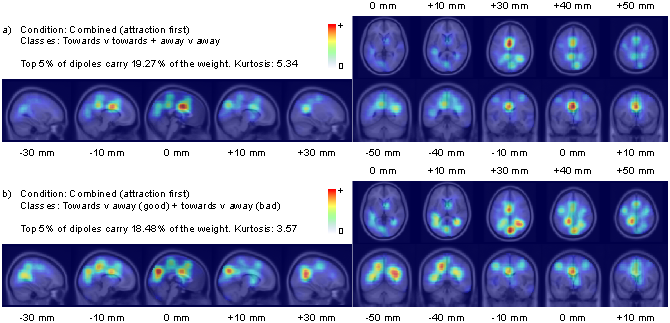
\includegraphics[width=\textwidth]{figures/salval-posfirst-wdd-combined-sum.pdf}
    \caption[Weighted dipole density plots of the combined salience- and valence-focused classifiers, for the attraction-first group.]{Weighted dipole density plots showing the relevance of cortical areas to \emph{a} the two valence-focused classifiers TvT and AvA, and \emph{b} the two salience-focused classifiers TvT+ and TvT--, both for the attraction-first group.}
    \label{salval:fig:posfirst-wdd-combined-sum}
\end{figure}

\clearpage 

Whereas the classifiers which combined valence and salience show three distinct cortical areas contributing to separability, the valence-focused classifiers focus almost exclusively on the mPFC region. The salience-focused classifiers on the other hand, isolate signals from all three regions identified earlier, but focus primarily on the central and lateral parietal regions.


\subsection{The Repulsion-First Group}
\label{salval:sec:results:repulsionfirst}%

Figure~\ref{salval:fig:negfirst-erp-channel} shows the grand-average ERP at Fz for the repulsion-first group. The same effects are visible as in Figure~\ref{salval:fig:posfirst-wdd-combined-sum} of the attraction-first group, albeit less pronounced. Following permutation tests with 10000 permutations, significant differences exist between 164 and 172~ms in the attraction condition. Around that same time in the repulsion condition, both classes show a slight negative deflection, where no significant differences can be reported. Figure~\ref{salval:fig:negfirst-wdd-combined-sum} shows the areas relevant to classification of the valence- and salience-focused activity. Unlike in the attraction-first group, no differences can be reported. Figures for the separate classifiers are included in the supplement.


\section{Discussion}

We presented an adaptation of the original implicit cursor control experiment \cite{zander2014implicit,zander2016nat} which allowed us to separate two dimensions that were originally coupled: salience and valence. Because they were originally coupled, it was unclear to what extent the reported results may have been influenced by perceptual processing of the movements, compared to the participants' valence-related interpretation of each movement. Here, stimuli were kept visually constant across two conditions in which valence was manipulated. This allowed valence processes to be targeted by comparing visually identical stimuli that had different valence, and perceptual (salience) processes to be targeted by comparing visually different stimuli that had the same valence. We hypothesised that, if the primary differences between the classes were to be valence-related, any effect seen within conditions would be inversed between them. Alternatively, there should not be any differences between the conditions if visual processing was the primary generator of such an effect. 

The `effect' in question can be most prominently seen in the ERP at channel Fz. The attraction condition accurately and significantly reproduced the positivity and negativity which indexed the different cursor movements in the original experiment. In the repulsion condition, however, we see neither an inversion nor a reproduction of this effect. Based on this, we can conclude that neither valence nor salience was the sole or primary generator of this particular effect, and indeed further analysis is required to disentangle their respective contributions.

Individually-calibrated classifiers offer a data-driven method to select relevant features from the available data; in our case, the ERPs across all channels between 0 and 600~ms following each cursor movement. The method presented in \citeA{krol2018classvis} allows these features to be localised in the brain, allowing the individual classifiers to be aggregated again across participants in 3D source space. Using this analysis, we see a focused selection of cortical areas that generate the differences between the classification schemes. We focused this analysis on the attraction-first group.

The mPFC was identified in the original experiment as the primary generator and remains prominent here. It points to the involvement of an error monitoring process, as per the reinforcement learning theory \cite{holroyd2002,nieuwenhuis2004rlern}. This is in line with the original interpretation of each movement as `feedback' which can be correct or in error depending on the expectations of the observer, or on the progress that the observer perceives towards the goal.

Since only the grid layout changed between the original experiment and the attraction condition, the increased involvement of the parietal lobe is likely due to the additional perceptual and spatial demands of the adapted grid. It is larger ($7\times7$ instead of the original $4\times4$), and the cursor's movements require additional spatial computation since the relative position of the reference node (the centre) changes more strongly than in the original experiment, where it always remained within one quadrant relative to the cursor. It is this additional computation that likely led to the increased involvement of this area, which is known to be involved in spatial processing \cite<e.g.,>{zipser1988,yantis2002parietalattention,goldberg2006saccadessalienceattention,silk2010spatialwmattention}.

Additionally, both the right-lateral inferior parietal lobule and a combination of the medial frontal and cingulate gyrus were identified by \citeA{dyson2015errorregions} as contributing to erroneous feedback detection, each ranking first, respectively, in two different methods quantifying their contributions. 

From among all the ICs present in the data, the various areas that the different classifiers focused on can thus be reliably related to the task at hand. More interesting is how they relate specifically to the dimensions manipulated in the experiment, and the different functional processes that would be present.

The original assumptions were formulated in the form of predictions or expectations being violated. The valence dimension was manipulated through the instructions, and created a tendency to predict the favourable outcome, i.e. that the cursor would move in the `appropriate' direction. The salience dimension could be interpreted as producing a similar tendency, except that it would preferentially predict that the cursor would move towards the visually salient point regardless of its valence. In this framework, the two predictions are congruent in the attraction condition, with these predictions either both being violated when moving away from the centre, or both being confirmed when moving towards the centre. If each final perception is referenced to both predictions separately and in parallel, with each prediction influencing the dopaminergic input to the mPFC accordingly, this would explain the effects observed at Fz. The congruent violations, each producing a negative deflection, would combine to result in a strong negative deflection as observed, while the strong positivity would reflect the congruent processing of `reward' for the two predictions. In the repulsion condition, the two processes are incongruent; where one would produce a stronger inhibition, the other would disinhibit the mPFC, and vice versa, essentially cancelling each other out. This is in line with the reduced negativities that are pronounced equally in both classes in Figure~\ref{salval:fig:posfirst-erp-channel} for the repulsion condition. 

An alternative account could interpret the negative deflections in the repulsion condition as an N2 component of the ERP, oft-reported to reflect a conflict monitoring process \cite<e.g.,>{nieuwenhuis2003conflictn2,yeung2004}. It largely matches the latency, spatial properties, morphology, and even cortical generators of the feedback negativity, so it cannot be uniquely differentiated from the feedback negativity in the present context---although there are reports that the feedback negativity itself results from conflict monitoring \cite{botvinick2001conflictmonitoring,yeung2004} or is at least sensitive to conflict \cite{jia2007perceptualconflict}. In the current experiment, the presence of a conflict-related process may however be postulated given the experimental design and the reported results. As mentioned above, in the repulsion condition, the salience and valence dimensions are incongruent, i.e., they are in conflict. In the attraction-first group, this may be exacerbated by participants possibly having been primed by the previous condition. Instead of the feedback negativity or reward positivity, a smaller negative deflection is seen reflecting this conflict between either the two predictions mentioned above, or the task parameters more generally. This, too, could explain the ERPs in Figure~\ref{salval:fig:posfirst-erp-channel}. The presence of conflict processing would additionally explain the tendency towards slower reaction times in the repulsion condition, reported for conflict conditions in general \cite{vidal2020errorsactionmonitoring}. 

This latter account, in its simplest form, does not include any effects on the ERP of valence or salience per se in the repulsion condition and focuses merely on conflict. A final account could be a combination of the two above, or the latter account with additional, unspecified processes related to these dimensions. Conflict processing could delay these more specific processes to varying degrees making them difficult to analyse using ERPs. Instead, such processes may be picked up by the classifiers which are individually calibrated and take single-trial variability into account.

Importantly, none of the possible accounts of the data presented above would invalidate the separation of the valence and salience dimensions by the TvT, AvA, TvA+ and TvA-- classifiers as explained in Section~\ref{salval:sec:methods:classification}. If the two processes exist separately in parallel as per the first account, the TvT and AvA classifiers average out the salience violations/confirmations and focus only on valence-related processes, while the TvA+ and TvT-- classifiers do the opposite to focus on salience. In the second account, these cross-condition classifiers would focus on the differences between the relevant process in the attraction condition, and this uniform conflict process. This would not interfere with the conclusion: If indeed the response processing is the same in both classes for the repulsion condition, it would serve as a neutral reference against which to compare the responses in the attraction condition. As such, the concept of salience- and valence-focused classifiers remains valid---although it would introduce additional relevance weights in the region responsible for processing the conflict. Alternatively, if the repulsion condition does additionally have valence/salience processes, or if any combination of the given accounts applies, similarly, a combination of the above two arguments applies and the concept of salience- and valence-focused classifiers remains valid.

We may thus focus on interpreting the differences observed between the classifiers as presented in Figure~\ref{salval:fig:posfirst-wdd-combined-sum}. As mentioned in Section~\ref{salval:sec:results:classvis}, the attraction-first group shows different cortical areas responding to salience and valence. The salience-focused classifier, which in this context should focus on differences with respect to the perceptual (visual) processing of the stimuli, is indeed localised primarily in the parietal areas identified earlier. The additional but weaker mPFC involvement points towards the involvement of either the conflict monitoring process mentioned above in the latter accounts, or the general (prediction) error system whose activity would remain relevant as per the first account.

In line with our hypotheses, the valence-focused classifier carries very little weight in the occipital/parietal regions, and is instead principally focused on the mPFC region, where EEG correlates of both error and reward processing have been postulated to originate \cite{holroyd2008rewardpositivity}, supporting that the feedback-related negativity is indeed at least partially reflective of valence \cite{yeung2004passiveactivefrn}.

The repulsion-first group, however, did not show this same pattern. Here, all classifiers were dominated by the involvement of a larger, less distinct parietal region. This does not rule out that the same patterns do exist in the data---indeed, the other measures do not differentiate this group from the other, and conclusions drawn on the basis of ERP and behavioural analyses apply equally to both groups. The difference in the relevant cortical areas however suggests that this group had a fundamentally different approach to the tasks in both conditions. It appears that the two conditions here cannot effectively be counter-balanced as intended, instead resulting in what are essentially two different experiments. Still, as a last validation, Figure~\ref{salval:fig:allparticipants-wdd-combined-sum} shows the valence- and salience-focused classifier localisation as applied to the data for both groups together. The conclusion as mentioned above with respect to the differential involvement of parietal and prefrontal cortical areas can still be drawn, with the different classifiers predominantly focusing on different areas. In the combined data, however, we also see the consistent involvement of an additional parietal area in both classifiers, an area which we now know to be explained by its exclusive presence in the repulsion-first group. As such, the separation of the two groups in this analysis helped sharpen the results. It also highlighted the importance of investigating the cortical origins of classifiers, a step which is often omitted.

We have shown that both salience and valence, i.e., both the visual properties of the presented stimuli as well as the subjective interpretation of these stimuli, play a role in the implicit cursor control paradigm as presented here and used before \cite{zander2014implicit,zander2016nat}. Furthermore, classification schemes can be developed to focus primarily on one or the other aspect. The differential processing of these aspects is supported by their different cortical origins.

Now taking a wider perspective, we wish to come back to the implications of the present results for neuroadaptive technology. The unit of analysis in this paper was the individual cursor movement, which was classified on single-trial basis. Single-trial classification allows the classifier output to be used in real time as input to a computer, e.g., to enable control. This control can be implicit if the brain activity that is being classified is not consciously or voluntarily modulated by the human. Implicit cursor control is an interesting case in that it demonstrates that the task of moving a cursor, which is a quintessential example of explicit control, can in fact be performed implicitly without participants being aware of doing so \cite{zander2014implicit,zander2016nat}: indeed there was no conscious or voluntary manipulation of brain activity that helped steer the cursor. When control or interaction happens unbeknownst to the users themselves---the ones supposed to be in control---the exact cognitive and affective processes that a classifier can potentially access make a profound difference with respect to the forms of interaction and the types of application that can be realised. The current results support the position that classifiers can access both perceptual processes, potentially allowing brain-as-a-sensor applications to be developed, and valence-related processing, i.e. cognitive processes that reveal subjective value judgements of the users. This latter category enables, among other things, unique forms of personalisation that may greatly increase productivity, but, given the deeply personal nature of the brain activity, may at the same time introduce particularly severe issues with respect to privacy \cite{mecacci2019criteria}, data security \cite{fairclough2014confidential}, informed consent, and outcome responsibility \cite{krol2020cognitiveprobing}. While we are looking forward to the further exploration of the possibilities of neuroadaptive technology, the current results emphasise that researchers and developers should take these potential issues into account. 


\section*{Acknowledgements}

Part of this work was supported by the Deutsche Forschungsgemeinschaft (ZA 821/3-1). 


\section*{References}

A shared bibliography starts at page~\pageref{bibliography}.

\vfill

\begin{figure}[!h]
    \centering
    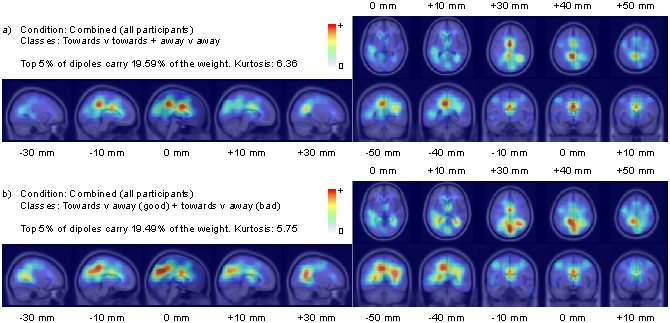
\includegraphics[width=\textwidth]{figures/salval-allparticipants-wdd-combined-sum.pdf}
    \caption[Weighted dipole density plots of the combined salience- and valence-focused classifiers, for all participants combined.]{Weighted dipole density plots showing the relevance of cortical areas to \emph{a} the two valence-focused classifiers TvT and AvA, and \emph{b} the two salience-focused classifiers TvT+ and TvT--, for all participants, i.e. combining both attraction-first and repulsion-first groups.}
    \label{salval:fig:allparticipants-wdd-combined-sum}
\end{figure}

\vfill\null

\clearpage
\begin{figure}[t]
    \centering
    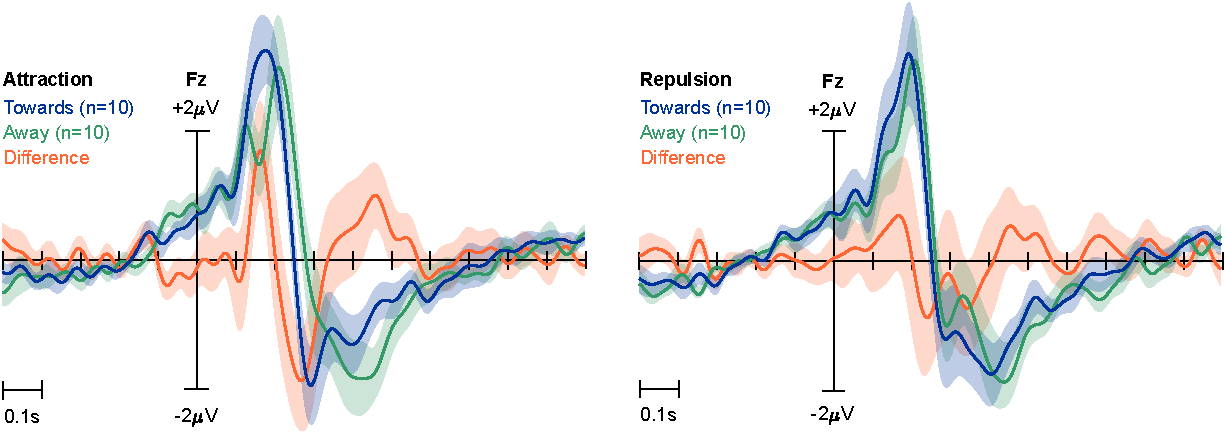
\includegraphics[width=\textwidth]{figures/salval-negfirst-erp-channel.pdf}
    \caption[The grand-average ERPs at Fz for the two conditions in the repulsion-first group.]{The grand-average ERPs at Fz for the two conditions in the repulsion-first group.}
    \label{salval:fig:negfirst-erp-channel}
\end{figure}

\begin{figure}[b]
    \centering
    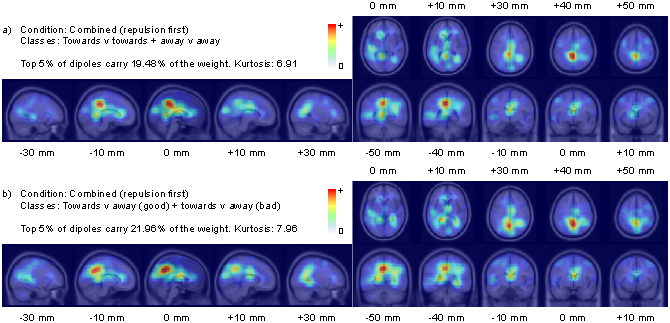
\includegraphics[width=\textwidth]{figures/salval-negfirst-wdd-combined-sum.pdf}
    \caption[Weighted dipole density plots of the combined salience- and valence-focused classifiers, for the repulsion-first group.]{Weighted dipole density plots showing the relevance of cortical areas to \emph{a} the two valence-focused classifiers TvT and AvA, and \emph{b} the two salience-focused classifiers TvA+ and TvA--, both for the repulsion-first group.}
    \label{salval:fig:negfirst-wdd-combined-sum}
\end{figure}




\clearpage
\pagestyle{empty}
\null\cleardoublepage
\pagestyle{plain}
